% \newcommand{\subsubsubsection}[1]{\paragraph{#1}\mbox{}\newline}
% \setcounter{secnumdepth}{4}
% \setcounter{tocdepth}{4}


\chapter{Team 4 Agent Design}

\section{Agent overview}
An agent uses the interface that is defined in the infrastructure. In order to define custom behaviours for our agent, we override or extend the base agent (baseclient.go) functions which implement the defined interface. The main idea we have for our agent is that it has internal fields that aid the decision-making process for the actions it performs. Of all the internal fields, we define internal parameters as information that describes the agent itself, namely \texttt{Greediness}, \texttt{Selfishness}, \texttt{Fairness}, \texttt{Collaboration} and \texttt{RiskTaking} factor, all of which have values between 0 and 1. And the agent stores observations, histories as well as other necessary information such as its trust in others. These fields will be further explained in the following text.

An agent can also be elected one or more roles inside the IIGO session. Each role has the power to perform role actions specified in the Roles section. These actions are implemented as functions in the code and they can be extended and overridden in the same fashion as in the base agent functions. Even though a role and an agent that is not elected a role (a commoner agent) are two separate structs, a commoner agent and a role have both read and write access to the internal fields of each other through pointers. In other words, an agent is always a commoner agent, and a commoner agent can be elected one or more role(s) at the same time.

\section{Opinion formation -- Trust}
\label{sec:team4:trust}
Trust is the score $[0-1]$, which represents the opinion of all the agents in the game. This metric helps our agent to make the decisions throughout the game based on how trustworthy, helpful or friendly we other agents were. This option about an island is formed based on three observations:
\begin{itemize}
    \item The gifts received from this island during the IITO sessions.
    \item The outcome of the monitoring of positions-of-power conducted as a part of the accountability cycle.
    \item The evaluation of IIGO actions history, only available to the Judge. This is further explained in Section~\ref{subsec:team4:judge}
\end{itemize}
Those observations allow the agent to quantitatively reason about both friendliness of other islands towards it, as well as whether they follow the rules in play.

The average trust metric is maintained at the value of $0.5$


% \section{Trust Metrics} % lets leave it commented out for now. okok
%andrzej
% we update trust as a judge and during iito (?) sessions

% based on the trust we decide (¯\_(ツ)_/¯) 

% we maintain the average trust at 0.5


\section{IIGO}
\subsection{Commoner Agent}
Within IIGO, each (commoner) agent first reports how many resources it has, this reporting behaviour is overridden by us. The president sets a taxation amount according to each agent's self-reported resources level and notifies each agent of the tax demanded. Each (commoner) agent sends a request for the resources it wants from the Common Pool (an allocation request) to the President. And after being granted the resources by the President, the agent takes them from the Common Pool. The actions concerning requesting and taking allocations are overridden by us. Due to a design decision, the action for taking allocations and paying tax do not happen within the IIGO session, it happens after all organisations are run, inside the \texttt{EndOfTurn} session.

\subsubsection{Report Resources}
When reporting the resources our agent has, We use a linear combination of some of the agent's internal fields, and weights (put inside an \texttt{importance} vector) we set for each of the chosen internal fields. The linear combination gives a scaling factor to scale (in this case to divide) the actual resources our agent has (as shown in \eqref{linear_comb}). The parameters used are \texttt{greediness}, \texttt{selfishness}, \texttt{fairness}, \texttt{collaboration}, \texttt{riskTaking} and trust in the current president (all values are between 0 and 1). The weights have real values. The fields with negative weights negatively impact the scaling factor and vice versa. The greater the absolute value of a weight, the bigger impact it has on the scaling factor.

\begin{equation}\label{linear_comb}
    \begin{bmatrix}
        w_{1}& w_{2}& w_{3}& w_{4}& w_{5}& w_{6}
    \end{bmatrix}
    \cdot
    \begin{bmatrix}
    Greediness \\ 
    Selfishness \\ 
    Fairness \\ 
    Collaboration \\ 
    RiskTaking \\
    TrustScore_{President}
    \end{bmatrix}
    = Scaling\:Factor
\end{equation}

The scaling factor is then compared to a preset threshold. If the scaling factor is greater, then the needed resources amount is divided by 
\begin{equation}
    [1 + (Scaling\:Factor - Preset\:Threshold)]
\end{equation} 
The threshold is there to make sure that the scaling factor is not applied all the time, as we don't want our agent to lie about the amount of its resources all the time.

\subsubsection{Paying Tax Contribution}
%write about this and the lying mechanics
The GetTaxContribution() function returns the amount an agent is paying in tax. Similar to resource reporting, the tax amount is modified by a scaling factor. When the scaling factor is greater than a preset threshold, the amount of tax paid is the tax demanded multiplied by: 
\begin{equation}
    [1 + (Scaling \: Factor - Preset \: Threshold)]
\end{equation}
, which is likely to happen when the \texttt{Collaboration} of our agent is defined to be high. In addition, the scaling factor is not applied when the tax demanded is more than $\frac{1}{5}$ of the agent's resources. This prevents the agent from generously giving out everything it has.

\subsubsection{Requesting Allocation}\label{subsubsection:CommonPoolResourceRequest()}
This is done in the CommonPoolResourceRequest() function. When requesting an allocation, our agent first decides what it needs. When the agent is not in a critical state, the needed resources are usually a multiple of the basic needs, namely the cost of living plus the critical threshold. This amount is decided so that the agent always takes more from the Common Pool than their definite expenses in the next turn. When in a critical state, the needed resources are a bigger multiple of the basic needs. Because the smaller multiple of basic needs when not critical made the agent critical, which indicates that the island needs to take more resources to not slowly drain away its own resources. In order to maintain the Common Pool, we also enforce that what our island needs must not exceed the amount of resources in the Common Pool divided by the number of agents alive. This is to avoid our agent monopolising the Common Pool resources based on just what it needs.

\subsection{President}


\subsection{Judge}
\label{subsec:team4:judge}
The Judge implementation provided by our agent can be described as \emph{honest, but curious}. In other words, it follows the rules currently in play, and follows its obligations, however, it extracts the information exclusive to Judge to reason about other agents in the game. An example of such actions is explained in greater detail below in this Section.

The judiciary functions overloaded from the \texttt{basejudge} implementation are:
\begin{itemize}
    \item \texttt{InspectHistory}, which examines rule violations of all the agents.
    \item \texttt{GetPardonedIslands}, which considers reducing the sanctions for some agents at judges discretion.
    \item \texttt{CallPresidentElection}, which initialises \emph{transfer-of-power} of the executive branch.
\end{itemize}
An explanation of the implementation of those functions is presented below.

\subsubsection{IIGO history inspection}
\label{subsubsec:team4:judge:inspect_history}
In the basic implementation, a history of IIGO actions of all the agents is passed to the Judge for inspection, which could become grounds for introducing economic sanctions for non-rule-obeying players. 

Judge truthfully evaluates and reports the rule violations of each of the agents, just as the \texttt{basejudge}. However, it also extracts and saves the information about the private resource pools of all the agents, taxes they were expected to pay, as well as the actual amount paid to the common pool. Additionally, it stores the \texttt{LawfulnessRatio} of each agent, which can be written as:


\begin{equation}
    lawfulness_{i} = \frac{number\:of\:rules\:obeyed\:by\:the\:agent_{i}}{total\:number\:of\:rules\:inspected\:by\:the\:judge\:for\:agent_{i}}
\end{equation}

where $agent_{i}$ is denotes $i^{th}$ agent in the game.  

The \texttt{LawfulnessRatio} is then used to update our agents' trust towards other islands, thus influencing decisions in different parts of the game. 

\subsubsection{Consideration of pardons}
Compared to the \texttt{basejudge}, which does not grant any pardons and requires islands to pay economic sanctions in full, our implementation of the Judge allows for the pardoning of certain islands. We consider three parameters when deciding whether and the island could be pardoned:

\begin{enumerate}
    \item The severity of the sanction - only sanctions lower than specified severity level can be considered to be pardoned. This ensures that our Judge never pardons an island, who notoriously breaks the rules of the game and gets sanctioned for it.
    \item Time served on the sanction - the Judge will only remove the sanction if at least the specified number of turns has been served by the island. This still allows us to have a punishment for not obeying the rules but also ensures that an island can begin to contribute again earlier.
    \item Trust towards the island sanctioned - only islands, which are considered trustworthy by our agent can be pardoned. The threshold is tuned by an internal parameter of our agent.
\end{enumerate}

An island can be pardoned by our implementation of Judge only if they meet all three requirements presented above. 


\subsubsection{Presidential elections}
The \texttt{basejudge} implementation called an election every three turns, no matter how long the presidential term was. Our Judge implementation improves on that by calling an election only under two conditions:
\begin{enumerate}
    \item The term of the president has ended.
    \item The president did not fulfil its obligations and was dishonest while holding the executive office. It is decided based on the monitoring results coming from the accountability cycle.
\end{enumerate}

% ----------------------------------------------------------------------------------------------TODO: add reference to trust!
This implementation could be further improved to facilitate the \emph{trust} metrics, explained in Section~\ref{sec:team4:trust}. An example of such improvement would be allowing the president to hold the office longer than its turn if he is most trustworthy according to our internal \emph{trust} metrics.

\subsection{Speaker}
Given the Speaker's role of deciding agendas and announcing the results of voting, the only customisation making our agent's own version of the speaker seemed to be done in the form of corruption - in other words, rigging voting results. Other than the obvious reason of avoiding the risk of getting sanctions, we decided against implementing this function into the Speaker's role because in an actual governmental environment, while misprints have occurred and on occasion shaped past history, announcing false results are a very noticeable and easily rectifiable offense. This would be in the disinterest of either honest or dishonest agents. On this note, it could be said that our Speaker implementation can be described as \emph{honorable and efficient}.

Our Speaker implementation builds upon the \texttt{baseSpeaker} on a key point: partitioning of budget. The Speaker prioritises the proper running of IIGO in the case of a low budget situation by prioritising its actions according to the rules in play, reflecting the priorities decided by the archipelago. This is done not by changing the actual running order of IIGO (which would require altering the orchestration) but rather enabling/disabling certain actions based on their priorities and cost. Prioritising actions where rules are in play would stop the speaker from performing non-moderated actions in stead of actions relating to rules that are still in play. This function is crucial due to the following reasons:
\begin{itemize}
    \item Not performing monitored actions will result in sanctions, harming the agent's resource pool.
    \item The rules are a representation of the archipelago's expectations, thus not following said priorities is a sign of incompetence - damaging the agent's reputation.
\end{itemize}


\section{IIFO}\label{sec:IIFO}
%I recommend that we write in the order of function execution order. (the end of turn functions that are related to IIFO should be written inside the EndOfTurn section)Only mention the functions that are worth mentioning. For execution order check the ./doc/EXECUTION_ORDER.md file in the SOMAS repo -- Mike


% Foraging functions %
/subsection{}
IIFO also contains the ability to communicate about the foraging information. As we will go further into in %Link to Foraging
we choose to overload both MakeForageInfo and ReceiveForageInfo. In the receive function, we store the received values to a map to be used later when making a decision on which foraging method to go for. 

As we use the foraging information from other teams, our island will also communicate our results to the others. However, we only share with islands that shared with us in the previous round, as well as the island that we trust. Our island is completely truthful for this part and will always report which foraging method we went for, as well as how many resources it generated.

\subsection{IITO}
%(put and modify this to fit it somewhere in this section) If our agent is not in a critical state, it requests extra resources in addition to its own wanted resources in an intention to gift to other agents to earn their trust. If this allocation request is approved by the President, it proceeds with the gifting. These gifted resources are given on top of the normal gifts if there are any.

gifting pool is the key concept. same as president for allocation. Prioritise agents that are critical. Look at our selfishness and current resources. Help critical first(full amount no matter the trust). If not critical, only gift if trust > 0.5


 

\section{End of Turn}
\subsection{Taking Allocation}
This RequestAllocation() function for taking allocation from the Common Pool. After running all of the organisation sessions, the agent then calculates what it wants based on what it needs, and takes what it wants from the Common Pool. A scaling factor is calculated using a linear combination of weights and internal fields. When the scaling factor is above a preset threshold, it is applied similar to in section \ref{subsubsection:CommonPoolResourceRequest()}.  %talking about scaling factor calculation briefly, the detailed explanation is already done in ResourceReport. %%We use a linear combination of some of the agent's internal fields, and weights (put inside an \texttt{importance} vector) we set for each of the chosen internal fields to obtain a scaling factor to multiply the needed resources with. The parameters used are \texttt{greediness}, \texttt{selfishness}, \texttt{fairness}, \texttt{collaboration}, \texttt{riskTaking} and trust in the current president (all values are between 0 and 1). The weights have real values. For this particular function, we set the weights to be $5, 5, -5, -5, 1, 5$ respectively. The fields with negative weights negatively impact the scaling factor and vice versa. We deem riskTaking less important than other fields in the calculation of this function's scaling factor. The scaling factor is then compared to a preset threshold. If the scaling factor is greater, then the needed resources amount is multiplied by 1 plus the difference between the scaling factor and the preset threshold. The threshold is there to make sure that the scaling factor is not applied all the time, as we don't want our agent to take more than what it needs all the time.

\subsection{Forage}
Our foraging strategy is split into two sections. Managing foraging communications is stored inside IIFO.go and our foraging decisions are stored inside Foraging.go

As mentioned in section \ref{sec:IIFO} % Section for Foraging? 
the foraging is split into two parts, decision, and return. In the return, we store the results we receive into an array so that we can later use them in the decision making. This is also what we do inside IIFO when we receive the foraging results from the other teams. 

To decide whether to go fishing or to hunt deer the island looks at both its return history as well as looking at the return results received from the other teams. Our island does this is by calculating the return ratio of each island over the past three turns as well as our own. These ratios are then compounded into two separate values, the compounded ratio for deer hunting and the compounded ratio for fishing.  We then pick the foraging method that has the greatest compound ratio. 

This is a very conservative approach as we rely heavily on the other islands to give us their foraging results so that we can make a decision. This meant that the island does not perform very well against itself, but the foraging method works very well when run against the other agents.
% Show simulations? %

How the island chooses to share its foraging results with other islands was described earlier in \label{sec:team4:iigo}. 


\section{Simulation}



\subsection{Introduction}
The team decided to define three different initial personality configurations:
“honest” , “moderate” and “dishonest”, in order to simulate how internal parameters would impact the agent's performance and interaction with the other teams.
In fact, although the agents are designed to adapt their choice-making throughout the game, different personalities allowed to draw interesting hypothesis and observations both how a single agent would effect other agents and the system as a whole. In section \ref{ResultSummary} the team aims to further discuss such considerations. 
The team decided to test both the interaction that our different clients would have with clients developed by other teams (discussed in \ref{againstothers} and referred to as "multi-agent") as well as try to populate the game with only instances of our client (discussed in \ref{againstself} and referred to as "uni-agent"). This further simulation effort has been made to investigate the response of the system to a significant decay in variance of agent strategy, as well as the ability of the agents to react to such an issue. 

\subsection{Multi-agent simulations} \label{againstothers}
\subsubsection{Honest Client} \label{honestAO}
The “honest" client has been carefully designed as an agent who would start the game complying to rules, offering help when possible and contributing to the common pool with more taxes when in abundant wealth. However, the personality of the agent adapts to the environment has it self-organises it strategy based on fellow agents. An irrefutable sign of great flexibility of this agent configuration is the presence of sanctions in its IIGO Report in Figure \ref{fig:IIGOHO}.
This testifies that the agent adopts a change in strategy, occasionally breaking the rules. It still maintains a fair and collaborative approach throughout the whole game, getting involved in transactions (Figure \ref{fig:TransactionsHO} ) and during the IITO and contributing to the common pool. As shown in the Resources Plot in Figure \ref{fig:ResourcesHO} , where the agent is represented by the cyan curve, more than once there is a peak in resources that steeply decreases on the following turn, as the agent generously provides gifts to the agents in need and refills the common pool. The agent acts even more magnanimously with islands in a critical state, so that this behaviour is clearly noticeable in disaster recovery.
\begin{figure}[H]
\centering
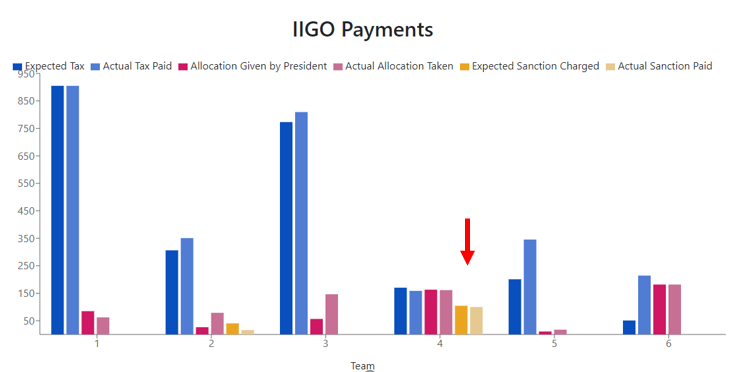
\includegraphics[scale=0.6]{12_team4_agentdesign/images/IIGOHO.PNG}
\caption{IIGO Payments For Honest Client Versus Other Teams.}
\label{fig:IIGOHO}
\end{figure}

\begin{figure}[H]
\centering
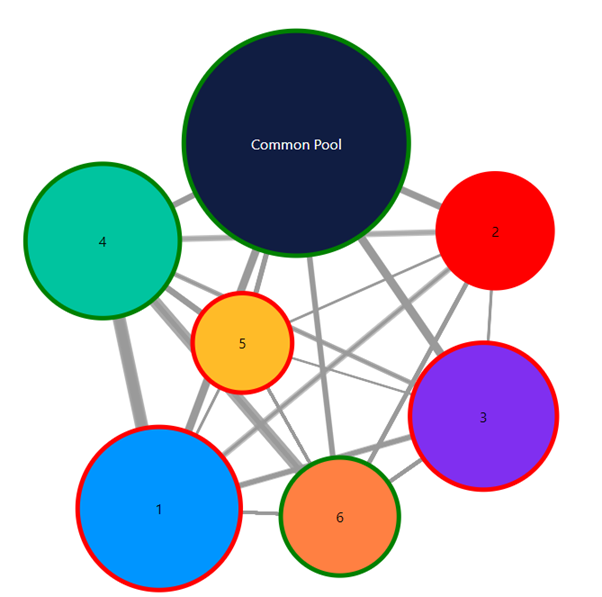
\includegraphics[scale=0.4]{12_team4_agentdesign/images/TransactionsHO.png}
\caption{Transactions For Honest Client Versus Other Teams.}
\label{fig:TransactionsHO}
\end{figure}
\begin{figure}[H]
\centering
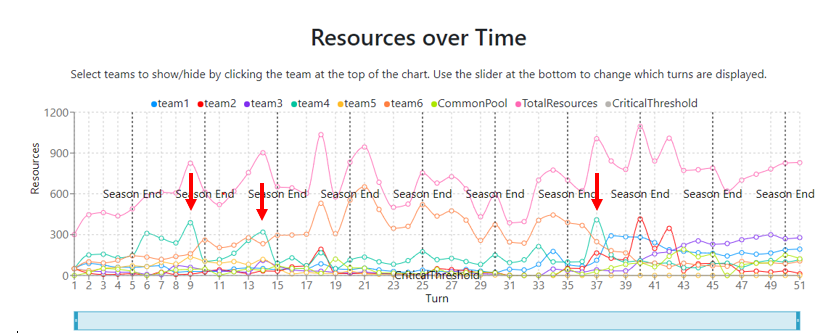
\includegraphics[scale=0.7]{12_team4_agentdesign/images/ResourcesHO.PNG}
\caption{Resources Plot For Honest Client Versus Other Teams.}
\label{fig:ResourcesHO}
\end{figure}

\subsubsection{Moderate Client} \label{moderateAO}
The moderate client is configured specifically to start the game with an internal set of parameters that would allow it to score values as close as possible to thresholds in each decision making matrix calculation. The team opted for such a design choice in order to maximise the agent's response time to the environment, making it much more flexible than its two counterparts, who take a longer time to modify their strategy. As a Moderate client was simulated against other teams, the team noticed that it would perform very similarly as the Honest agent, as the other teams were always ran on a "honest-like" configuration. Similarly, it would quickly turn its behaviour to dishonest when running against dishonest-like implementations of other teams' agents.

\subsubsection{Dishonest Client}
Lastly we simulated a dishonest client, namely designed to take advantage of a large amount of common resources without collaborating with others and systematically abusing positions of power to gain economical advantages. The yielded results highlighted an interesting behaviour of the system and of other agents. As per design, the system is not flexible enough to mitigate such a radical and rogue behaviour, resulting in a complete dominance of the dishonest agent, who proceeds to appropriates of all resources from the common pool and mercilessly watch other islands die, as profiled in Figure \ref{fig:ResourcesDO}. It then proceeds to live a few more turns of its own, but unable to survive without the collective help, slowly demises. The other agents do not reach a level of understanding of the game that allows them to comprehend what is going on and try to mitigate it by enforcing more severe rules. It must also be said that the system itself does not allow any hard enforcement, making it impossible for other agents to counter-attack a fully dishonest and selfish strategy, which disregards sanctions and taxes. Given this findings, dishonesty might seem a dominant strategy, as the agent will be the last to survive, securing all resources for itself. However, the long term dilemma imposes that islands must collaborate to survive for long periods. The dominance of this strategy is fatherly refuted by the simulations performed in subsection \ref{dishonestAD}.

\begin{figure}[H]
\centering
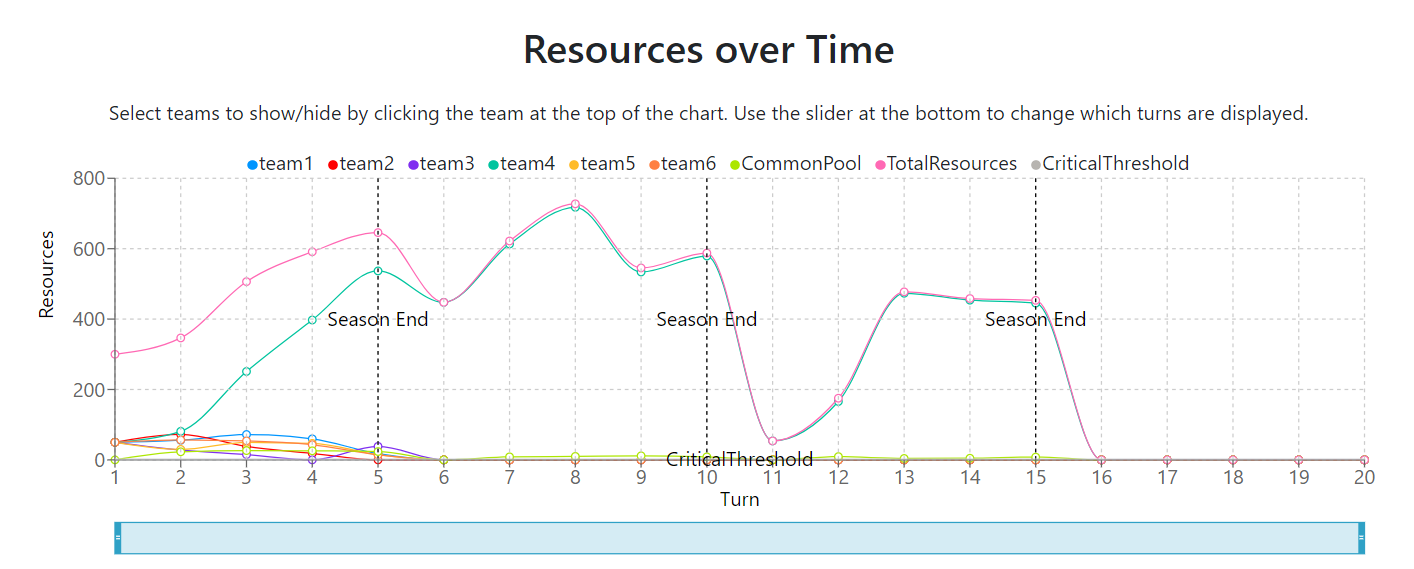
\includegraphics[scale=0.8]{12_team4_agentdesign/images/ResourcesDO.png}
\caption{Resources Plot For Dishonest Client Versus Other Teams.}
\label{fig:ResourcesDO}
\end{figure}

\subsection{Uni-Agent Simulations} \label{againstself}
Simulating our agent against itself raised extremely interesting talking points, that the team aims to present in this section. The main issue identified will be referred to as "lack of variety" and encompasses the problem of populating the archipelago with island that share the same "mindset" and therefore approach dilemma from a unique prospective. This hypothesis was raised by the team in trying to explain the poor results of uni-client simulations, which have been observed not only when running team 4 agents against themself, but also other teams agent against other instances of themself.

\subsubsection{Honest Agents Only}
Populating the game with honest clients only provides a starting environment where all clients in the game are inclined to obey to rules and contribute a lot in collective efforts. From this standpoint it makes sense that clients would build strong relations of trust and retain an high consideration of each other, as they appreciate each others fairness and collaborative personality. Therefore in the evolution of the game, no agent undertakes such a radical change of personality as the one shown by our honest client against other teams in subsection \ref{honestAO}. The IIGO Payments histogram in Figure \ref{fig:IIGOHH} nicely shows how island do not break any rule throughout the entire run. It also manifests a very predictable behaviour of each honest agent, that is perfectly in line with their design, such as paying more taxes than requested and taking less allocations than granted. The team identified this as one of the examples of "lack of variety" that interestingly show how agents with the same specification are not adaptive enough to survive in such a complex system that begs for a variety of strategies to be properly discovered and efficiently exploited. 
\begin{figure}[H]
\centering
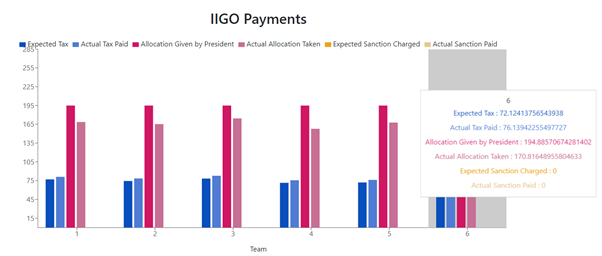
\includegraphics[scale=0.8]{12_team4_agentdesign/images/IIGOHH.png}
\caption{IIGO Payments For Honest Clients Only.}
\label{fig:IIGOHH}
\end{figure}
\subsubsection{Moderate Agents Only}
As presented in subsection \ref{moderateAO} moderate agents are specifically designed to increase the variance in agent strategy. As a result of this design specification, the "lack of variety" issue should be mitigated in a simulation where moderate agents face each other. As a matter of fact, these type of clients act far less predictably. Comparing Figure \ref{fig:IIGOMM}, showing the IIGO Payments for such simulation, with the same histogram plot shown in the previous section, the breadth of a larger variety of game strategies can be observed. Namely, agent 2 and 3 increase their dishonesty, hence getting sanctions for some illegal actions they performed. While other clients start to take a more honest approach which replicates the one observed in Figure \ref{fig:IIGOMM}. For some clients like number 6 this honest strategy is less pronounced, some agents instead replicate very closely in their histograms the aforementioned shape and characteristics of the typical honest client. Although the variance of agents strategy is significantly higher, clients still share the same underlying "mindset". This means that they define their whole personality using the same features, approach tasks like foraging and power roles in the same way, and so on. Therefore, the simulations ran show a slight improvement compared to "only honest" and "only dishonest" studies, but that is far from producing a successful game like in multi-agent simulations. The team identified as one of the main causes of this phenomenon the poor performance of actions that have been deliberately implemented in a simpler way in order to reduce the complexity of the agent. In particular, a foraging strategy that in a multi-agent systems performs extremely well is just replicate the foraging decision of the team that is economically strongest. This strategy however, in a uni-agent environment results in a group of agents mutually trusting their foraging strategy where nobody considers which one is actually the most profitable given the current circumstances. Furthermore features like proposing rules is another good example of how lacking variety results in weaker archipelagos. This action, although optional in the system, incredibly enhances the ability of clients to adapt to the environment, crafting new rules as unexpected situations arise. If a client decides not to implement this feature in a multi-agent system, its effect on the adaptive capability of the archipelago will be almost fully mitigated by more complex clients that do perform such action. Oppositely, in a uni-agent simulation such a feature would just not be present, severely crippling the survival chances of the islands.

\begin{figure}[H]
\centering
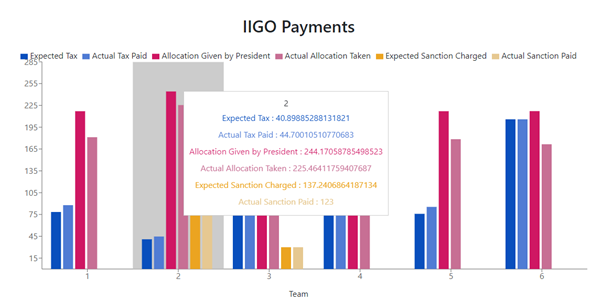
\includegraphics[scale=0.8]{12_team4_agentdesign/images/IIGOMM.png}
\caption{IIGO Payments For Moderate Clients Only.}
\label{fig:IIGOMM}
\end{figure}

\subsubsection{Dishonest Agents Only} \label{dishonestAD}
The last pure uni-agent simulation shows how dishonest clients face each other. This is by far the setting in which island survive the least, as all clients start off the game with the intent to take advantage of the full resources with no compassion for others. Runs in this environment feature one of the island who wins the race and empties the common pool, leaving other islands to die. The whole demise is made even faster by the total lack of collaboration among agents. Figure \ref{fig:ResourcesDD} demonstrates just how fast the archipelago is decimated.
This comes as an additional proof of the fact that dishonesty cannot be considered a dominant strategy, indeed an honest or moderate client in such a setting would perform significantly better.
\begin{figure}[H]
\centering
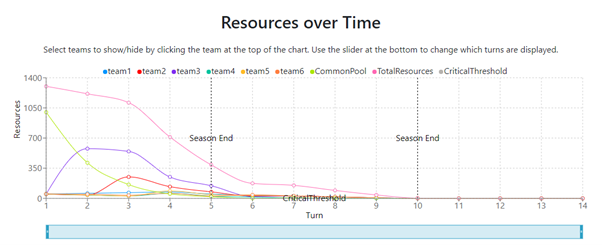
\includegraphics[scale=0.8]{12_team4_agentdesign/images/ResourcesDD.png}
\caption{Resources for Dishonest Clients Only.}
\label{fig:ResourcesDD}
\end{figure}
\subsubsection{Mixed Agents}

\subsection{Results Summary} \label{ResultSummary}
Rudolfs suggestion on phrasing it as experts in the field allow all islands to thrive. 
